
\documentclass[review,12pt,authoryear]{elsarticle}

%% The amssymb package provides various useful mathematical symbols
\usepackage{amssymb}
%% The amsthm package provides extended theorem environments
%% \usepackage{amsthm}

%% The lineno packages adds line numbers. Start line numbering with
%% \begin{linenumbers}, end it with \end{linenumbers}. Or switch it on
%% for the whole article with \linenumbers.
\usepackage{lineno}

% for adjusting table width automatically
\usepackage{adjustbox}
\usepackage{tabulary, ragged2e}
\usepackage{booktabs}

% Below is Elseviers requirements - they are similar to most articles and a good point of reference when writting scientific articles or analyses in general.
%1.Full Length Article A full-length article should be a substantial and in-depth research study regarding a particular state of issue through several techniques or approaches. 
% The main text should be approximately 6,000 words in length, but it should not exceed 8,000 words (excluding abstract, references, tables, figures, and appendices).
%A maximum of 250 words abstract and up to 10 displayed items (figures and tables) is allowed. A full-length article should include an Introduction,
%Materials and methods, Results, Discussion, Conclusions, and References, which can be accompanied by Supplementary material.

\begin{document}
\begin{linenumbers}
\begin{frontmatter}

%%%%%%%%%%%%%%%%%%%%%%%%%%%%%%%%%%%%%%%%%%
%%       Start Matter      %%
%%%%%%%%%%%%%%%%%%%%%%%%%%%%%%%%%%%%%%%%%%

%% Title, authors and addresses

%% use the tnoteref command within \title for footnotes;
%% use the tnotetext command for theassociated footnote;
%% use the fnref command within \author or \affiliation for footnotes;
%% use the fntext command for theassociated footnote;
%% use the corref command within \author for corresponding author footnotes;
%% use the cortext command for theassociated footnote;
%% use the ead command for the email address,
%% and the form \ead[url] for the home page:

%% \title{Title\tnoteref{label1}}
\title{An analysis of interrelations between economic and environmental variables in Australian Winegrowing.}

% Variable importance in determining vineyard operational costs and region using statistical machine learning.
% How are region and operational costs related?

% Regional differences in Australian winegrowing (Quality)?

%% \tnotetext[label1]{}
%% \author{Name\corref{cor1}\fnref{label2}}
%% \ead{email address}
%% \ead[url]{home page}
%% \fntext[label2]{}
%% \cortext[cor1]{}
%% \affiliation{organization={},
%%      addressline={}, 
%%      city={},
%%      postcode={}, 
%%      state={},
%%      country={}}
%% \fntext[label3]{}

%% use optional labels to link authors explicitly to addresses:
%% \author[label1,label2]{}
%% \affiliation[label1]{organization={},
%%       addressline={},
%%       city={},
%%       postcode={},
%%       state={},
%%       country={}}
%%
%% \affiliation[label2]{organization={},
%%       addressline={},
%%       city={},
%%       postcode={},
%%       state={},
%%       country={}}
%\affiliation[label1]{organization={QUT},
% addressline={},
% city={},
% postcode={},
% state={QLD},
% country={}}
%\affiliation[label2]{organization={AWRI},
% addressline={},
% city={},
% postcode={},
% state={SA},
% country={}}
%\affiliation[label3]{organization={Food Agility CRC},
% addressline={},
% city={},
% postcode={},
% state={Vic},
% country={}}
\author[label1,label2,label3]{Author}
\date{02/08/2023}

% \begin{abstract}
% \end{abstract}
%%Graphical abstract`
%\begin{graphicalabstract}
 % \includegraphics{graphical_abstract.jpeg}
%\end{graphicalabstract}'

%\begin{keyword}
%% keywords here, in the form: keyword \sep keyword
%Keyword one \sep{} keyword two
%% PACS codes here, in the form: \PACS code \sep code
%\PACS{} 0000 \sep{} 1111
%% MSC codes here, in the form: \MSC code \sep code
%% or \MSC[2008] code \sep code (2000 is the default)
%\MSC{} 0000 \sep{} 1111
%\end{keyword}
%%Research highlights
\begin{highlights}
 \item Highlight 1
 \item Highlight 2
 \item Highlight 3
 \item Highlight 4
\end{highlights}
\end{frontmatter}

%%%%%%%%%%%%%%%%%%%%%%%%%%%%%%%%%%%%%%%%%%
%%        main text       %%
%%%%%%%%%%%%%%%%%%%%%%%%%%%%%%%%%%%%%%%%%%

\section{Introduction}

%%%%%%%%%%%%%%%
% Paper setup %
%%%%%%%%%%%%%%%

% Why is the question/issue/problem worth examining?
There is a lot of economic pressure on Australian winegrowers and the wine and vine industry in general due to international market changes, tighter requirements for organic and sustainability credentials and a shrinking market.
% FIXME: Get some references in here!



 There is a need for increased understanding of different underlying conditions leading to improved performance in agricultural productivity and sustainability \citep{oecdInnovationProductivitySustainability2019}.

 Specifically within the Australian Vine and Wine industry there is a need to further understand the driving relationships between resource use and economic output .
 Environmentally sustainable
 UC Davis in California has created a new green-tech winery, a sustainable entity and blueprint
 on how to differentiate a brand. Growers need to determine better and efficient ways to make
 wine, develop benchmarks with local growers and market this approach. \citep{lukemanciniUnderstandingAustralianWine2020}


% What is the context for your reserach?
An unprecedented amount of data regarding the Australian wine and vine industry has been collected through Sustainable Winegrowing Australia offering new insights into the driving economic forces of the Australian wine industry.

% What do you want to achieve?
We hope to uncover the driving relationships and factors of economic sustainability in Australian Winegrowing. 

% Are there any relationships you want to explore?
We explore the relationship between various operational and resource use variables to operational costs and vineyard gross margin.

%%%%%%%%%%%%%%%%
% Working title
%

% Description
% NB Avoid titles along the lines of: “Effects of ...”, “The role of ...”, etc.  Be specific about the effect and its significance so that your reader knows what is on offer.
%  TODO:

% For example, rather than write a title like “The effect of factor X on astrophysical properties of green cheese.”, 

% be specific about the effect and write something more like ...

% “Factor X halves the lunar thermal diffusivity of  green cheese”.

% You will usually find it easier to write an effective title if you make your title a sentence.

% Notes
% N/a

%%%%%%%%%%%%%%%%%%%%
% Intended readers
%
% Agricultural economists
% Growers
% Property managers (beyond winegrowing)
% Mardi seemed super interseted - I know a lot of growers would be interested, however I am not sure of any names in particular beyond the usual cases such as Hans, David Klassen etc.
% Perhaps those seeking to purchase a property.

% Description:
% Name 4 or 5 potential readers - give their names and why they would be interested  (e.g. “Ichabod Crane, paleo-fudgologist interested in polygalactic fudginomiality”, not “assorted paleo-fudgologists”).   

% Your readers should be outside your institution.

%%%%%%%%%%%%%%%%%%%%%
% Anticipated Journal
%
% Wiley Journal of Agricultural Economics
% https://onlinelibrary.wiley.com/journal/14779552

% Descrption
% Ensure that all readers are likely to read the nominated journal  (e.g.  few non-researchers read refereed academic journals; politicians simply don’t read). 

% Notes
% Contributors to the JAE should note that, in choosing subjects for articles, the objects of the Society are ‘to promote the study and teaching of agricultural economics and relevant disciplines, and their application to issues in the agricultural, food and related industries, rural communities and the environment. The relevant disciplines include economics, statistics, marketing, business management, politics, history and sociology'. Preference will be given to articles which deal either with new developments in research and methods of analysis, or apply existing methods and techniques to new problems and situations which are likely to be of general interest to the Journal’s international readership. The Journal is not a suitable publication for articles of purely local interest.  Articles should be clearly and concisely written and should normally not exceed 7,000 words. Articles greatly in excess of this limit cannot be considered for publication.
% 
% A definition of agricultural economics from the encyclopedia britanica:
% 
% agricultural economics, study of the allocation, distribution, and utilization of the resources used, along with the commodities produced, by farming. Agricultural economics plays a role in the economics of development, for a continuous level of farm surplus is one of the wellsprings of technological and commercial growth.

We study the economic outcomes of Australian vineyards and their statistical relationships to the utilisation of the resources used. This is done through analysing a new comprehensive nationwide data set using XGBoosted models. We further compare the relationships between different resources to address the extensive collinearity found within the data. XGBoosted models were used because they are able to overcome multicollinearity as well as highlight the level of importance that predictor variables have; with importance being able to be statistically defined through different measures. 

applies existing techniques to a new data set 

agricultural economics and relevant disciplines, and their application to issues in the agricultural, food and related industries, rural communities and the environment. The relevant disciplines include economics, statistics, marketing, business management, politics, history and sociology'. Preference will be given to articles which apply existing methods and techniques to new problems and situations which are likely to be of general interest to the Journal’s international readership. The Journal is not a suitable publication for articles of purely local interest.  Articles should be clearly and concisely written and should normally not exceed 7,000 words. Articles greatly in excess of this limit cannot be considered for publication.

%%%%%%%%%%%%
% Question %
%%%%%%%%%%%%

% Things to consider
%
% Why is the knowledge important?
A better understanding of driving economic factors within agricultural industries helps to drive sustainability through understanding relationships between factors better.
%  FIXME: work on this^ 

% What is the significance?
This broad dataset has not yet been analysed, showing new insights into the driving factors of the Australian winegrowing industries economy

% How will the findings be utilised?
These findings can be used by growers and property managers to help understand the driving factors that affect their operational costs and gross margins.

% What improvements may be derived from this result?
These insights help to optimise the gross margin and minimise the operational cost of a vineyard.

% Are the terms well defined?
% Some terms need more definition.

% Is it doable? (cost & ethics)
%  ITs done!
%       Can you finish it in time?
% Do experts think your question is important/relevant/doable?
%  Mardi was pretty excited about it!

% What is the nature of your question?
%         who, what, where, when, why, how?
The primary nature of this question is what, and then how: What are the driving factors for operational cost? And, how do these factors relate to each other?

% You can have more than one question.

% What is the most important question your paper will pose?
What are the driving factors for operational cost and gross margin in Australian Winegrowing?

%
% NB It is essential that your answer is framed as a direct question.  Your response must end with a question mark.



% Briefly outline the problem you are tackling and explain why the problem is important to knowledge in general.  “Nothing much is known” is not sufficient justification by itself.  You have to show why the gap in knowledge is important. Expect to draw heavily on your reading of the literature in framing your answer but do not get into detail of  author and year.
% 
% ^ is this almost boiler plate writing at this point. Considering that not much is known but we are applying it in a specific field, in this case to economics. We can use a general, nothing is known but further understanding this for economic reasons will help to improve the economic sustainability of these practices. and that these authors have postulated about these connections etc. We can start generic and funnel it into the reasoning of importance using the journals general frame work and objectives.

%%%%%%%%%%
% Answer %
%%%%%%%%%%

% What is the answer to question
Region is a driving force in determining profits.
Fuel and water are the primary driving operational costs

%
% 
% NB  You must give a direct answer to the question posed.
% Notes

% Will the findings be considered significant?
The finding themselves are not that significant, it is the evidence of a complex system governing these relationships that is the significant finding.

% How did you gather the evidence? 
%
% Briefly outline the methods you used to gather your evidence.
They were gathered by Sustainable Winegrowing Australia

% What is the main evidence?
%
% Briefly outline the key results.  Focus on outcomes.

% What can you add to theory?
%  
% A research paper has to add to broader understanding. What will yours contribute?  Think about how your results and conclusions will change how people see the world.
What we add is that agricultural economics maybe complex systems that are obfuscated by the expertise of growers to navigate problems such as drought, pests and disease. These systems, although predictable through some variables are not causal. We see this in the evidence of some years not affecting outcomes even though they are known to contain the aforementioned issues. % TODO: use the evidence of draught to be an example. Show why year should be important but is not!

%
% Many people have trouble with this section.   Do not recycle the results.  Focus on the conceptual models that explain why your results are as they are, or why they are different from what might have been expected.  Your contribution may be something new or it may be confirmation of something already known but in a slightly different context.
%
% Sometimes the contribution to theory is not a simple answer but a better understanding of the questions that ought to be asked in future.
%
% Again, expect to draw heavily on the literature in framing your answer, but cite the literature only sparingly here (you can go into full detail when you prepare your discussion).

% What can you add to practice?
%
% Superior research also has practical consequences.  What are the consequences of your work?  Think about how your results and conclusions might change what people do. Do not merely restate your results.
It maybe better to pursue more causal models and create decision support systems than to model factors directly. It is difficult to untangle the predictive and correlative nature of the variable compared to the causal reasons.

%%%%%%%%%%%%%%%
% Future work %
%%%%%%%%%%%%%%%

% What remains unresolved?
% 
% You may or may not have a lot to say here.  Some of it may be useful in your discussion.
The causal reasoning behind these variables behaviours. The untangling the multicollinearity of these variables.
% FIXME:
% Whats been done? Whats the persistant gap? Why is a data-driven approach the answer?
A data driven approach can highlight the significance between different factors. And, highlight how heavily these factors relate through their relative importance.
% Predictive Modeling: When the research goal involves making predictions or forecasts, a data-driven approach, particularly using machine learning algorithms, can analyze historical data to build predictive models. These models can be used to make future predictions or test hypothetical scenarios.
% Exploratory Research: When the research area is relatively unexplored, and there is limited theoretical framework or prior research to build upon, a data-driven approach can help in exploring patterns, trends, and relationships in the available data. This can lead to the formulation of new hypotheses and research directions.
% Large and Complex Datasets: When dealing with large volumes of data that are too complex to be analyzed using traditional methods, data-driven techniques such as machine learning algorithms, data mining, or big data analytics can help in uncovering meaningful insights that might not be apparent through conventional approaches.

% TODO:
%  From the code comments~ We might want to show the relationship between revenue and operational cost! then we have an idea of how these two are related.
% # These are artefacts of. As profit can be negative it is harder to predict! We know after some further mapping that both operational costs and gross margin have a cubic root relationships to the logarithm of other variables. An interesting relationship to have!
% # 
% # Importantly this cubic root relationship exists between operational costs and gross margin, which is worth noting. However we want to know what tips it either side of them being equal as that shows that a vineyard is profitable!!

In the past decade, the Australian grape and wine industry has undergone a variety of pressures, including changing market demands, disease and drought \citep{wineaustraliaAustralianWineProduction2021}. Furthermore, natural resources are likely to decrease, as pressures from climate change increase, making it more important than ever to improve the efficiency and sustainability of crops \citep{agdeeNationalGreenhouseAccounts2021}. It has become crucial for those in the wine industry to address issues relating to environmental sustainability and economic viability, with a growing need for the industry to close the research gaps between sustainable practices and their real and perceived environmental and economic advantages \citep{montalvo-falconSustainabilityResearchWine2023,ouvrardDoesSustainabilityPush2020}. This paper aims to provide a comprehensive analysis of the intricate relationships between economic and environmental variables within the winegrowing sector. By employing statistical machine learning we show how interconnected vineyard variables are. Utilising a ten year data set that spans Australia we show the predominant 
elements in classifying region and year, % FIXME: A reader will ask: why would i want to predict region and year?
 as well as determining a vineyards potential operational costs and profit.
\par
This analysis utilises 
XGBoosted trees % FIXME: Why XGBoosted trees?
 to classify region and year; and to determine operating cost and profit of Australian vineyards. Classification and regression trees are 
 utilised as surrogate models %FIXME: Why are we utilising surrogate models?
to shed insight into the key partitions used by the XGBoost ensembles. Variable importance is further used to illustrate the 
interconnectedness % FIXME: What kind of interconnectedness?
of the different predictor variables, and to show the similarity in
variable importance % FIXME: What does variable importance mean in this context?
between different response variables (particularly between region and operational cost). This study aims to assist in uncovering 
the complexity of variables %FIXME: This is too vague, what makes them complex? why are the complex? etc
that are affected by a variety of vineyard management decisions to illustrate 
complex interplay of variables. % FIXME: What do you mean by complex interplay? Like what? An example?
This study endeavours to gain insight into the 
similarity % FIXME: Why do we want to know the similarity?
 in predictor variable importance between year, region, operational costs and profit.

% Initiatives to improve the environmental impacts of the Australian Wine industry have been ongoing since the 1990s; with recommendations to implement strategies for national programs that would help educate industry members in sustainable practices (Keith Jones, 2002). The first legislative initiative to support national programs was the Environmental Management Guidelines for Vineyards in Western Australia during 2002 (Nind, 2002). The first national program was the Australian Wine Industry Stewardship, beginning shortly after, during 2004 (WFA, 2009). This program was replaced multiple times during the 2000s, first by the Australian Wine Environmental Stewardship, and then by EnviroWine, finally becoming EntWine in 2009. The period in the 2000s was further influenced by several key researchers and program leaders, where concurrently multiple regions developed approaches to sustainable management tied to sustainability programs (SWA, 2023). EntWine was eventually acquired by the Australian Wine Research Institute and Australian Grape & Wine during 2015; which would lead to its redevelopment into Sustainable Winegrowing Australia (SWA) during 2019/2020 (SWA, 2023).
%             2.1.2. Previous Research and Motivation
% During the period of 2010 to 2023 data was collected voluntarily from wine industry members through the national sustainability programs, ultimately being in SWA possession as of 2023. The data set was used in 2020 to analyse sustainable practices, resulting in the development of a Resource Intensity Score (RIS); where the RIS was a summary indicator value of a vineyard’s energy use, emissions and water use (Nayak et al., 2020). The analysis then fit vineyards’ RIS values to 55 variables sourced from 23 separate wine regions during the period of 2015 to 2018 through the use of Stepwise Regression modelling. It was found that the top 10% gross margin vineyards had a lower operating cost and a lower RIS score than vineyards in the bottom 10% gross margin.
% The motivation for this thesis is to investigate the differences between the top 10% gross margin vineyards and those of the bottom 10%, hoping to uncover what the key differences were and to relate them to sustainable practices; as there is a known gap in the literature due to the difficulty to evaluate relationships using empirical evidence of both the environmental and economic impacts of sustainable practices in viticulture. This difficulty stems from data scarcity, industry complexity and transparency. While there have been attempts to fill these gaps, methodologies and indicators have lacked in ability to compare different regions and scales (Baiano, 2021).
%             2.1.3. Economic Pressures
% Historically strong demands for Australian wine have helped to create a thriving industry, however recently sharp reductions in exports to mainland China due to significant deposit tariffs have caused  a decline of 19% in Australian export value during the 2021-2022 financial year (see Figure 1) (Wine Australia, 2022). The pressure brought on by the drop in export value has been exacerbated by loss of tourism and labour due to the COVID-19 pandemic, global freight crisis, war in Europe and rising inflation (Wine Australia, 2021a, 2020). These pressures within the wine industry have trickled down to vineyards, where winemakers retain unwanted wine, creating an oversupply of grapes. Currently the proposed strategy to soften pressures proposed by Wine Australia includes initiatives focused on market diversification, and sustainability to build resilience in the coming years. 
% Figure 1:  The exports of Australian wine over time in Australian Dollars Free On Board, comparing exports between China and the rest of the world. This graphic is taken from the Wine Australia Annual Report of 2020-21(Wine Australia, 2022).
%             2.1.4. Environmental Pressures
% There are several environmental concerns that affect viticulture, including loss of soil quality, lack of rain, hail, disease, fire, and frost; with climate change exacerbating these issues. In 2020, 40,000 tonnes of grapes were lost across 18 different wine regions due to bush fires and smoke taint; the predicted incidence of wildfires is expected to increase (Canadell et al., 2021). In comparison to countrywide pressures such as drought, this damage made up only 3% of the total amount of grapes for that year; although acknowledged as a considerable loss on an individual basis, it was deemed to be only a minor national concern by Wine Australia when compared to other environmental pressures such as drought (Wine Australia, 2020). 


% \if{false}

% We classify regions to find the most prominent and well-defined relationships to regions.
% We examine the variables that are the most decisive in determining region.
% We compare the similarities and differences of these regions
% - within the analysis and
% - within the literature (also in their definition and history)

% We examine the similarity between these classifications and the variables that are significant in classifying profitable vs not.
% How do regional changes affect that. What is similar and what is different.

% We can link these contributing factors back to the baselines - at least anecdotally, or in an unpublished section. This will be good for the thesis.

% \fi

% %%%%%%%%%%%%%%%%%%%%%%%%%%%%%%%%%%%%%
% The Australian wine-growing industry is a rich and diverse landscape that is separated into multiple Geographical Indicator Regions. Each region describing unique reputations, qualities and varietals of wine produced there. While a great deal has been done regarding individual regional properties and traits, there has been little statistical insight into broader regional comparisons; due to a lack of cross-regional and in-depth data sources \citep{keithjonesAustralianWineIndustry2002,knightFirmResourcesDevelopment2019}. In this study we use Classification Trees to compare regional differences and how these differences relate to sustainable practices. 
% \newline

%
%This analysis addresses the knowledge gap regarding the effectiveness of regional level strategies employed in the wine industry and their relation to grape quality.
% What the hell is a regional strategy
% And how do you define, or know what trategy each region is using?
%
% Through the use of classification trees this study aims to highlight the key differences in sustainable practices at a regional level and how these practices relate to the different grades of grape quality.

% This does not really address what the methods are - aside from classisifcation trees in the most vague sense.
% What are the results briefly? why should someone read this article?
% What is interesting - what will be discussed in the article with regard to these results? What makes me want to read the article?
% And what is the take away point of the article? If I cant be bothered to read this article, what piece of knowledge can you leave mewiwth that I could recommend the article to someone else with?

\section{Methods}

% FIXME:
% While overall this methods section seems technically correct, more work is needed on justification, motivation, and context.
% Through the methods, motivate each decision youve made with context from the particular problem/data/question. Why is the basic standard procedure not adequate? This helps to slow it down and help the reader understand complex methods.
%
% As kate put it in person you are currently writting like ||||| fact fact fact. You need to be more |...||...|| with context etc inbetween each fact so that people can digest it.

% As with the previous paper, put the models up front it is very unclear what you have created - and less clear to understand it if there is no way to reference to it.

% FIXME:
% In this methods section, what is novel/innovative? Not currently clear, In particular - if I gave this data & these packages to a 3rd year class, which part here couldn't they do?

% FIXME: The methods needs to be restructured. Try the following order:
%     - Why do it?
%     - What does it do? (at a high level)
%     - How did you do it?
% 
% You should also include subsections. I think subsections are a good crutch because they can always be removed if the flow is done well.
% 
% Avoid following a narrative. Do not do the who/what/when/where/how/why and the big reveal.
% An aside comment might be that you can attempt to follow the narrative writing paradigm across the paper as a whole but limit your methods section to the why, what then how. And use the results as your reveal.
% Or maybe dont do that - it might just be that you need to write it like a narrative as a first draft then butcher it into the necessary sections. That writing style is incredibly ingrained at this point.

% FIXME: Adde a section for CV.

% FIXME: Another section that needs to be added is one that describes what the sankey and chord diagrams are and what they represent. The reader needs to be prepped for this before the results. They need to be able to properly interpret them.

% FIXME: Explain how some variables are one-hot-encoded and how this relates to variable importance. This is a significant resulti n the xgboost tree for the huntervalley

% FIXME: the motivation is missing from methods.
% FIXME: What is interrelated importance?

\subsection{Data}

% 6091 samples - total
% 58 regions
% 10 years

% 853 with reported profits
% 46 regions
% reported since 2018
Data used in this analysis were obtained from Sustainable Winegrowing Australia. Australia's national wine industry sustainability program. The program aims to facilitate grape-growers and winemakers in demonstrating and improving their sustainability \citep{swaSustainableWingrowingAustralia2022}. Data recorded by the SWA is entered manually by winegrowers using a web based interface tool. A total of 6091 observations were collected from 2012/2013 to 2021/2022 financial years. 23 variables were used for each observation reflecting a vineyards account for the given year (see Table \ref{tab:vars}). 
The profit variable was transformed % FIXME: What was it before?
and included as another separate variable, profitable; depicting whether a vineyard was profitable or not.
\par

\begin{table}[] 
 \label{tab:vars}
 \caption{Summary of variables used in the analysis. The recorded column indicate the number of values that were either greater than zero or that were not missing.}\label{tab:summary}
 \begin{tabular}{@{}ccccl@{}}
  \toprule
  \textbf{Variable} & \textbf{Units} & \textbf{Recorded} & \textbf{\begin{tabular}[c]{@{}c@{}}Number of\\ Classes\end{tabular}} & \\ \midrule
  Water Used & Mega Litres & 5846 & & \\
  Diesel & Litres & 5585 & & \\
  Biodiesel & Litres & 25 & & \\
  LPG & Litres & 958 & & \\
  Herbicide Spray & Times per year & 2026 & & \\
  Year & Class & 6091 & 10 & \\
  Disease & Class & 6091 & 2 & \\
  Region & Class & 6091 & 58 & \\
  Solar & Kilowatt Hours & 622 & & \\
  Irrigation Type & Class & 6091 & 20 & \\
  Petrol & Litres & 4309 & & \\
  Slashing & Times per year & 2290 & & \\
  Yield & Tonnes & 5935 & & \\
  Irrigation Energy & Class & 6091 & 16 & \\
  Area Harvested & Hectares & 6091 & & \\
  Electricity & Kilowatt Hours & 1015 & & \\
  Insecticide Spray & Times per year & 1092 & & \\
  Fertiliser & \begin{tabular}[c]{@{}c@{}}Kilograms \\ of Nitrogen\end{tabular} & 795 & & \\
  Fungicide Spray & Times per year & 2260 & & \\
  Cover Crop & Class & 6091 & 32 & \\
  Water Type & Class & 6091 & 39 & \\
  Profit & AUD & 853 & & \\
  Operating Costs & AUD & 853 & & \\ \bottomrule
  \end{tabular}
\end{table}

The data originally contained only two multiclass variables: year and region. Variables that measured the same metric from different sources (such as water collected from rivers versus water from dams) were converted into multiclass variables representing the source. The total amount used from these variables was retained as a separate variable. Occurrences of multiple sources were defined as separate classes. 
\par
The variable region represented one of the 65 Geographical Indicator Regions (GI Region) used to describe different unique localised traits of vineyards across Australia \citep{hallidayAustralianWineEncyclopedia2009,oliverReviewSoilPhysical2013,soarClimateDriversRed2008}. Each region is explicitly defined under the Wine Australia Corporation Act of 1980 \citep{attorney-generalsdepartmentWineAustraliaCorporation2010}.
\par
%
% Mention one-hot-encoding.
%

%
% How deep into the classes do we go?
%
\subsection{XGBoosted Trees}
% FIXME: What do boosted trees do?
XGBoosted (eXtreme Gradient Boosting) trees were created using the XGBoost library \citep{chenXGBoostScalableTree2016} in the Python Programming language \citep{g.vanrossumPythonTutorialTechnical1995}. They were chosen for this analysis as they provide both a 
high predictive performance % FIXME: For what?
and ability to effectively 
capture complex relationships % FIXME: How?
. An XGBoosted tree was created for each variable to show how they interacted. Each tree included all but the economic variables (profit and operating cost), which were only included once as response variables.
% FIXME: what does this mean in terms of the method and outputs?
\par
Following Chen and Guestrin \citep{chenXGBoostScalableTree2016}, XGboosted trees predict a value $y_i$ from the input $x_i$. The method of prediction is achieved through a tree ensemble model, using $K$ additive functions to predict the output. 
% FIXME: All equations must be in the middle or end of sentances, not at the beginning.
\begin{equation}
 \hat{y_i}=\phi(x_i)=\sum_{k=1}^{K}{f_{K}(x_{i})}, \space f_{K}\in \mathcal{F},
\end{equation}

% FIXME: The methods would benefit from some subsections (signposts)
% FIXME: What does the equation do? Give intuition.

where each function $f_K$ is a classification or regression tree, such that all functions are in the set of all decision trees $\mathcal{F}$, defined by ${f(x) = \omega_{q(x)}}(q : \mathbb{R}^m \rightarrow T, \omega \in \mathbb{R}^T)$. 
Where, $f_K$ corresponds to an independent tree structure $q$ of $\omega$ weights. % FIXME: Sentance fragment.
Each tree has $T$ leaves, which contain a continuous score, represented by $\omega_i$ for the i-th leaf. 
The final prediction % FIXME: What is this?
is determined by the sum of the score of the corresponding leaves, given by $\omega$. 
The set of functions % FIXME: You haven't described the tree as having a set of functions?
%  I believe when you refer to the set of functions F you might benefit from putting the F in brackets here or being more explicit where the functions are.
used by the tree is determined by minimising the 
regularised % What is the regularised objective?
objective function, given by:

\begin{equation}\label{eqn:objective}
 \mathcal{L}(\phi)=\sum_i l(\hat{y_i}, y_i^{t-1} + f_t(x_i)) + \sum_k \Omega (f_K).
\end{equation}

The difference between the 
prediction and actual variable % FIXME: what are the predition and actual variables?
% When you are talking broadly about elements of xgboost I believe it will help to refer to the equation, an example or something more specific. This would help to address the other comment regarding giving an intuition to the method.
is a convex loss function $l$. To optimise $l$, the difference is calculated for the i-th instance at the t-th iteration. The function 
$f_t$ % FIXME: Kate asked if this was $f_K$. This is not the case as $f_K$ is part of the penalty function, and I know this at first glance due to working with the equation regularly for this paper. If Kate is confused about this then your explanation sucks. It is to obtuse, like Kate has said you are hitting people with too many facts and not padding it enough to the context of this paper and its application or even its purpose. The function $f_t$ is incredibly important, especially because for the purposes of this study it changes depending on the variable and its nature. You are clearly not 
is selected according to which value minimises (\ref{eqn:objective}). The model complexity is penalised by the function $\Omega$, this acts to smooth weights in an attempt to prevent over fitting.
\par
As predictions are made using additive tree functions, XGboosted trees can be used for classification and regression. Due to the mixture of continuous, binary and multiclass variables in this analysis, 
both classification and regression trees were created. % FIXME: What were these created for?
The difference between the trees created for this analysis was the objective function used. % FIXME: Kate marked this with a "?" clearly highlighting the issue with the previous comment regarding f_t (at some point was on line 321)
XGBoosted regression trees were created for continuous variables, using the 

% FIXME: The below section talks about the objective functions. Kate askes what they are and what they related to. You will need to go into the objective functions, how they are different and why different functions are required to be used.
% Perhaps a reference that talks about the importance of objective functions.
root-mean-square as the objective function. Binary class variables utilised the logistic loss function as the objective. And, Multiclass variable used the soft max function. All objective functions are defined within the SKlearn library \citep{sklearn_api}, linked via an API to the XGBoost library \citep{chenXGBoostScalableTree2016}.
\par
% FIXME: Why are you doing this? give me reasons related to this work to keep reading.
Chen and Guestrin \citep{chenXGBoostScalableTree2016} illustrate, using Taylor expansions, that for a fixed structure $q(x)$ the optimal weight $\omega^*_j$ for a leaf $j$ can be derived. Furthermore, they show the loss reduction after 
the split % FIXME: What is the split?
is given by the function:

\begin{equation} \label{eqn:enumerate}
\mathcal{L}_{split} = {{1}\over{2}} \left[ 
 {{(\sum_{i\in I_L}g_i)^{2}}\over{\sum_{i\in I_L} h_i + \lambda}} +
 {{(\sum_{i\in I_R}g_i)^{2}}\over{\sum_{i\in I_R} h_i + \lambda}} -
 {{(\sum_{i\in I}{g_i})^{2}}\over{\sum_{i \in I} h_i + \lambda}} \right] - \gamma,
\end{equation}

with the tree structure defined using left $I_L$ and right $I_R$ instance sets of nodes, with $I = I_L \cup I_R$. Instead of enumerating all possible tree structures, a greedy algorithm iteratively adds branches to the tree minimising $ \mathcal{L}_{split} $ in (\ref{eqn:enumerate}). The frequency of a variable's occurrence within a tree is directly attributed to the minimisation of the objective function (or loss) through the minimisation of $ \mathcal{L}_{split} $.
\par
% FIXME: The below section needs to come sooner
The frequency of a variable appearing as a node within the ensemble was used as a measure of importance. This measure was chosen as it connected a variable to the minimisation of its associated objective function, translating the value into a 
simple count metric. % FIXME: Variable importance might need to be in its own section to fully explain it and its motivation.
% FIXME: The creation of xgboost trees for each variable needs to be earlier and more clear as well contextualised by its motivation.
Creating XGBoosted trees for each variable allowed the use of importance to show how strongly variables were associated with each other. The importance of predictor variables to economic variables was illustrated through the use of 
Sankey diagrams constructed % FIXME: More needs to be said on this. More needs to be talked about regarding the chord diagrams as well. There is no thorough explanation of how the diagrams work and what you have done with them to fully explain them!
using the Holoviews python library \citep{philipp_rudiger_2020_3904606}. Other variable's interconnectedness was demonstrated through the use of a chord diagram also created using Holoviews. % FIXME: The above comment about sankey diagrams applies to chord diagrams. These need fuller descriptions.
\par
% FIXME: More info is needed regarding the validation and how it was performed. This section can be expaned on as different validation and scoring is used due to the differencein objective functions. This is a rather critical section and very little is said about it.
% 
Each variable utilised 80\% of the data to train the XGBoost ensemble, with 20\% reserved for testing and validation. Testing was done through the iterative minimisation of the respective objective function for the variables type. For continuous variables 20\% was used as testing data, minimising the root-mean-square function. The final model was validated using repeated k-fold cross validation for 10 folds, repeated 10 times. $R^2$ scores were used to determine the best regression models during validation.
For binary and multiclass variables data was split into 80\% training, 10\% testing and 10\% validation data. 
Due to class disparity in multiclass variables (most prominently in region) data was stratified % FIXME: What does it means to stratify the data and why is this done?
into each subset at the same ratio of class occurrence. Validation was summarised through the accuracy, the proportion of true negatives and positives.
\par
% FIXME: rewrite the below paragraph in the active voice.
The use of the XGBoost library incorporates regularisation techniques built into the software to mitigate over-fitting and enhance model generalisation. The further use of cross validated grid search functions allowed for the selection of better performing hyperparameters when selecting the final model. The performance measure for model selection was root-mean-square error for continuous variables. The receiver operator characteristic's area under the curve was used for category variables \citep{hanley1982meaning}. Multiclass variables utilised the one verse one approach to minimise sensitivity to class disparity \citep{ferriExperimentalComparisonPerformance2009,handSimpleGeneralisationArea2001}.
% FIXME: What is the output?
\subsection{Classification and Regression Trees} % FIXME: perhaps this should be renamed surrogate models
% FIXME: It is not clear what you are trying to achieve with these models. No where do you give a definition of what a surrogate model is and why you are using it!
% Be specific about the purpose of what these models are being used for! Justify why you have not simply shown one of the ensembles trees as well! The use of these algorithms means that the tree is more general than any one of the ensembles manifestations.
Classification and Regression Trees were created for region, year, profit and operating cost. These models describe the partitions that are useful in predicting these variables; giving insight into the trees that make up the ensembles created by XGBoost. These trees were created using the rparts and caret packages \citep{kuhnBuildingPredictiveModels2008,terrytherneauRpartRecursivePartitioning2022} in the R statistical programming language \citep{rcoreteamLanguageEnvironmentStatistical2021}.
\par
Decision trees were validated using K-fold cross validation. Each model was validated using 10 folds, utilising a random selection of different samples ten separate times to validate each of the decision trees. The same measure of accuracy as the XGBoosted trees was used for comparison.

\section{Results}

% FIXME: The first result should be in the langauge of the question. In the original document the first result presented was region, implying that the question is: 'are regions different?' which is not the forefocus of the article. The results need to be rearranged to show grossmargin and operating costs as more significant variables as they are the curious factors that we do not understand.

% FIXME: The irritating placement of the figures is due to the way latex uses the /ref function to determine where a figure should be. Have a google of this to overcome it as the figure placement is all over the shop.

\subsection{Region}
% FIXME: there are artifacts from the previous paper. Although the previous paper is pertinant to some of this (quite critically so) it is no longer the primary focus. On top of this some of these terms such as 'Region Classification' are not well defined. This is because previously a great deal of effort was put into defining them and describing the potential regions. However this has been removed.
% FIXME: This section is much more of a: 'isn't it weird?' That region is not as significant in some areas but not others. That is can be used to predict things like yield but no profit etc. This phrasing shows why it goes after other sections. if you are writting by significance then it is not a significant find but it is something that is worth noting - unlike year which was just oh dear we dont know what is going on.
Region classification performed % FIXME: what does this mean - see the above comment.
% Note that it is not about the implications but getting in the definition of these terms. These things should be prepared for the reader well before the results. There should be no new terms here, we should just be refering to the outcomes that were established in the methods, and they should already have their motivations and contexts estabished (there is more that Kate has written if you are confused this is my translation after our meeting).
at 32.34\% (3.67\% standard deviation) and 56.82\% accuracy (50.58\% validation accuracy), for the classification tree and XGBoosted ensemble respectively. The most prominent feature used to classify regions with the classification tree was water source (see Figure \ref{fig:region_tree}). This differed from the variables that illustrated the greatest importance for the XGBoosted ensemble (see Figure (\ref{fig:region_sankey}), with predictor variables being highly interrelated in importance. 
Area, water, fuel and yield were more determining factors when predicting region using XGBoost. % FIXME: Is this perhaps your primary test? The fact that Kate was asking this means that the tools you are using do not have a well defined purpose in this analysis. I believe this stems from the lack of contextual motivation behind these tools. What is it that you are testing? Why are these important? This problem is throughout the paper and cannot simply be fixed here.
Although water and diesel were two of the three most frequently occurring variables in predicting region, they were not as connected to the other predictor variables as Yield and area harvested were.
\par

Many of the regions had significantly lower reporting rates, resulting in much poorer classification performance. The regions with the most samples performed the best. Bordering regions were routinely grouped together and misclassified as the same region. Two areas that suffered the most from this, specifically with the classification tree were the Limestone Coast (cool coastal areas in South Australia) and the warmer inland regions along the Murray Darling. The classification tree likely had more difficulty discerning vineyards closer to the river using only water sources due to the greater access to river water in these areas.
%, for example the two closest regions to Coonawarra, Padthaway and Wrattonbulley, were misclassified as Coonawarra even though they had 147 and 137 samples respectively. The same case was found for the Murray Darling, with 143 samples, it was misclassified as the Riverland. These misclassifications are likely due to the incredibly similar regional properties and close proximity these regions have with one another. Other misclassifications were most likely due to lower reporting rates with many regions being under represented.

\begin{figure}
 \resizebox{\textwidth}{!}{
 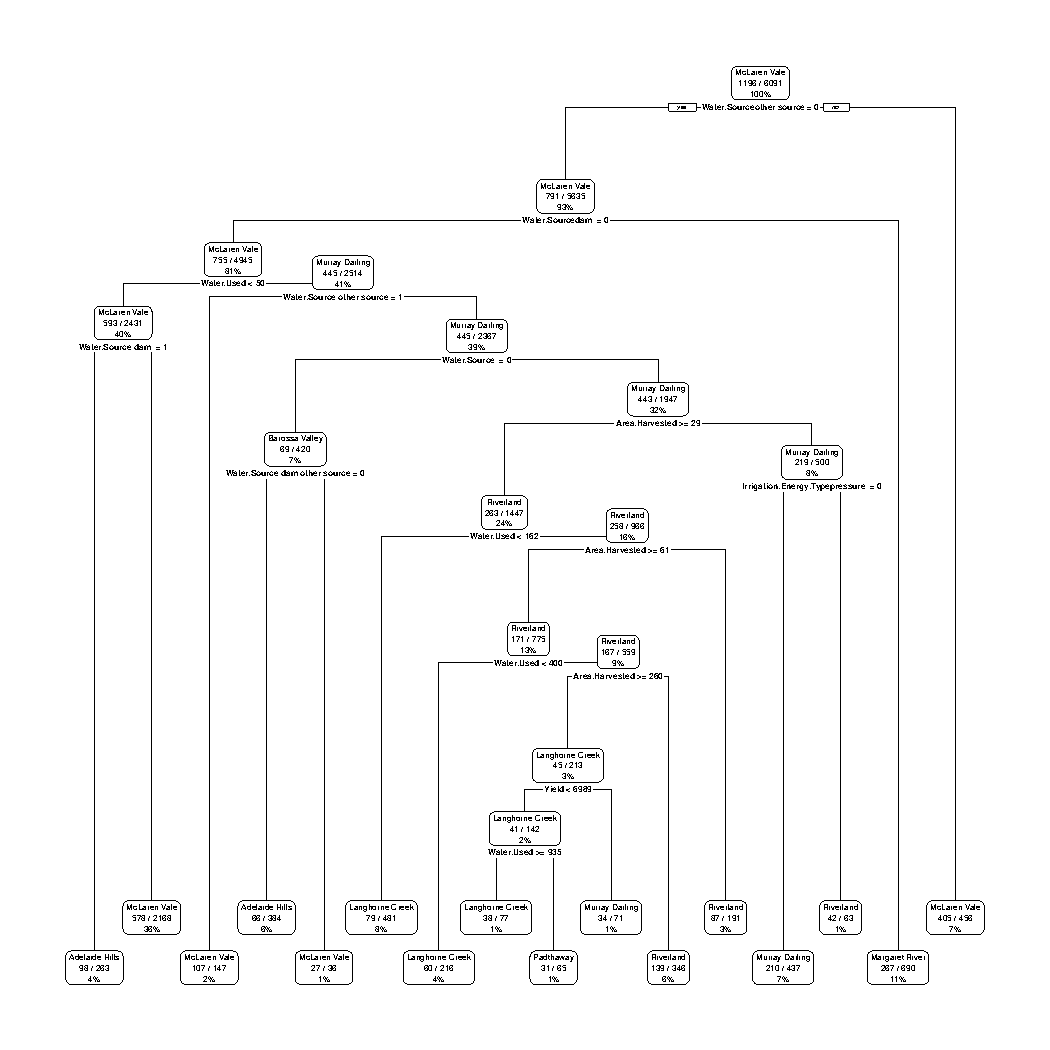
\includegraphics{region.pdf}}
 \caption{Decision tree predicting Region. Each node indicates the class predicted, and the proportion of elements agreeing with nodes partitioning, with the left direction indicating a yes to the nodes rule.}\label{fig:region_tree}
\end{figure}

\begin{figure}
 \resizebox{\textwidth}{!}{
 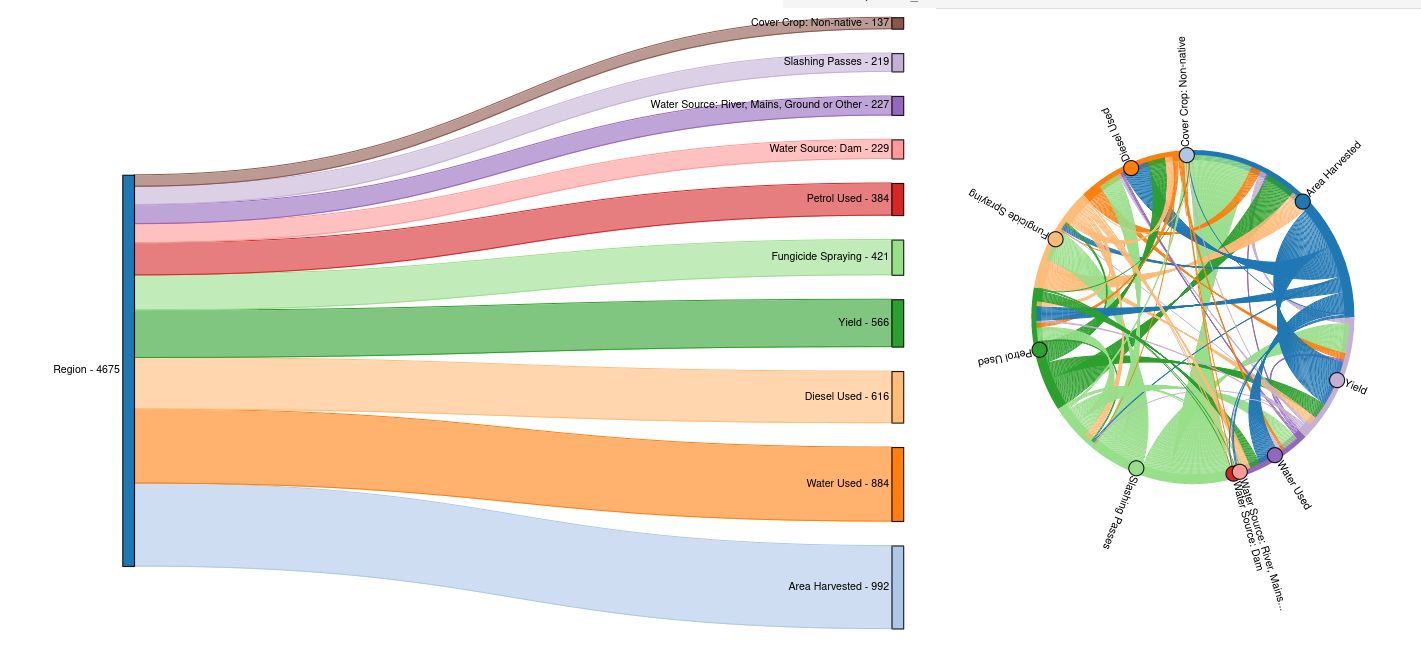
\includegraphics{region.png}}
% FIXME: What are the #'s? What do the sizes mean? What are the colours? What is interrelated importance?
% FIXME: Mark one Panel A and the other B
 \caption{The left-hand side depicts the 10 most important variables in predicting Region using XGBoosted trees as a measure of node occurrence, using a Sankey diagram. The right-hand side depicts the interrelated importance of the ten predictor variables using a chord diagram.}\label{fig:region_sankey}
\end{figure}

\subsection{Operating Costs}

% FIXME: Try to follow the same format for each of the section in the results. It will help to include a leading sentance about why the metrics are different everytime.

There was a pronounced difference in accuracy between the regression tree and the XGBoost model when predicting Operating costs. With the regression tree achieving an $R^2$ of 0.0931 (with a standard deviation of 0.0197) in its cross validation. The XGBoosted regression ensemble achieved an $R^2$ of 0.8025 (with a standard deviation of 0.1033).
\par
Within the XGBoost ensemble's nodes for operating costs (see figure \ref{fig:operating_costs_sankey}) fuel, water, area and yield occurred the most, similarly to region. Both diesel and petrol were of more relative importance (being ranked higher) in operating costs than water was compared with region. It is surprising that electricity, slashing and spraying passes was not more prominent in operating costs. 
% FIXME: Me and Kate talked about this. The diagrams, their context and justification go into the methods. How to interpret them needs to be better outlined here. You need to affirm peoples intition of them and the significance of more ribbons going out than in as well as why we are only using 10 variables.
However, Figure \ref{fig:year_sankey} shows that electricity, slashing and spraying are important variables in determining area and yield.

Electricity in particular is used predominantly for irrigation and so is related largely to the size of a vineyard. However, slashing and spraying are measured in discrete tractor passes and show a surprising connection to the overall size of a vineyard, despite not being scaled to any measure of size. This would mean that, although measured as the same increment, a slashing or spraying pass in a larger vineyard would consume more fuel and wages than in a smaller vineyard. % FIXME: May need to maintain bigger vineyards are more likely to have more staff verse small owner operators. Those extra staff may be trying to keep employers busy be sending them slashing (this comment was from Mardi and very hard to validate in the literature.)

%
% Is there any point in including this if its so bad?
%
% \begin{figure}
%  \resizebox{\textwidth}{!}{
%  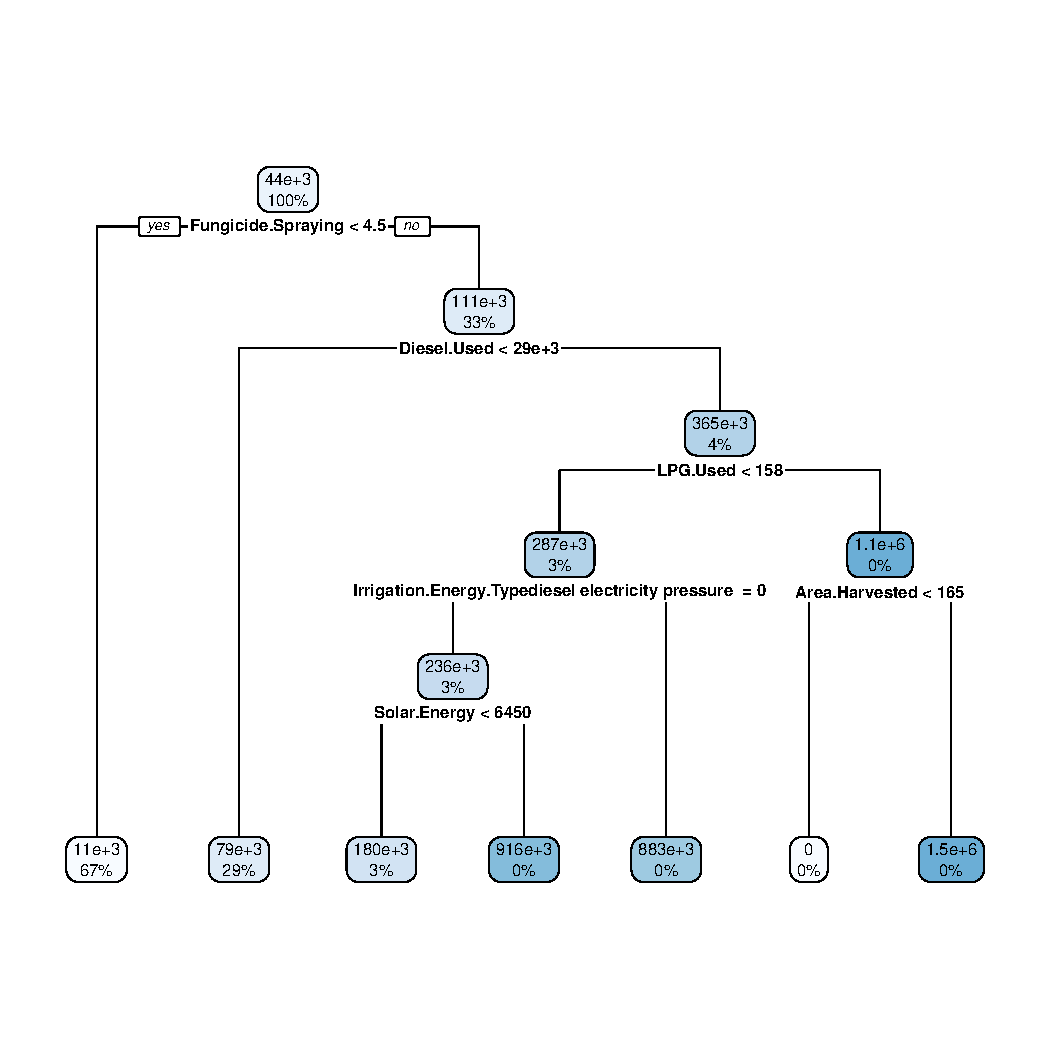
\includegraphics{operating_costs.pdf}}
%  \caption{Decision tree predicting Operating Costs. Each node indicates the class predicted, and the proportion of elements agreeing with nodes partitioning, with the left direction indicating a yes to the nodes rule.}\label{fig:operating_costs_tree}
% \end{figure}

\begin{figure}
 \resizebox{\textwidth}{!}{
 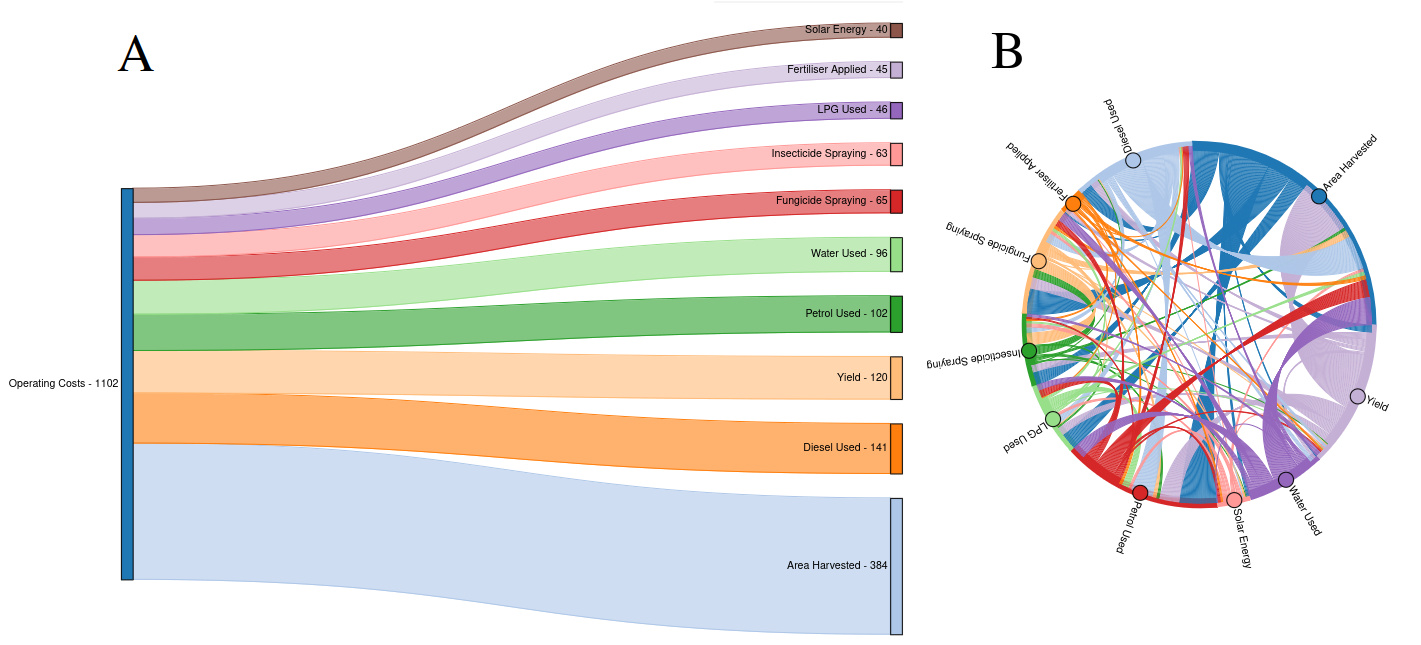
\includegraphics{operating_costs.png}}
 % FIXME: What are the #'s? What do the sizes mean? What are the colours? What is interrelated importance?
 % FIXME: Mark one Panel A and the other B
 \caption{The left-hand side depicts the 10 most important variables in predicting Operating Costs using XGBoosted trees as a measure of node occurrence, using a Sankey diagram. The right-hand side depicts the interrelated importance of the ten predictor variables using a chord diagram.}\label{fig:operating_costs_sankey}
\end{figure}

\subsection{Profit}

Predictions of profit performed poorly compared to operating costs with the regression tree having an $R^2$ of 0.1873 (with a standard deviation of 0.0522) and the XGBoosted ensemble achieving an $R^2$ of 0.2535 (with a standard deviation of 0.3126). The high standard deviation in the XGBoosted tree was a bias in more accurately predicting vineyards that made profit compared to those that lost money.
% FIXME: Kate pointed out that it is unclear what this implies (the below sentance).
% The following paragraph goes into it though, it would be better to meld these together. Talking more about the fact that it was easier to predict those who made a profit than those who did not.
% FIXME: It is wise to run a model purely on gross margin as well. It might have better insights than just profit! And it might over come this disparity.
With much higher $R^2$ values being achieved in k-folds containing only those that made profits (recording a maximum of 0.7634).
% profit summary stats
% max 3345000
% min -3937878
% std 396027.633119089
% range 7282878
\par
There was a disparity of 66.63\% of vineyards recording a profit than those that did not. When predicting if a vineyard would be profitable or not the classification tree and XGBoosted ensemble did not perform considerably differently from this proportion. With the regression tree achieving an accuracy of 68.66\% (and a standard deviation of 0.01\%) and the XGBoost ensemble achieving 71.97\% accuracy (with a validation accuracy of 70.59\%).
\par
It was surprising that operating costs performed substantially better in $R^2$ compared to profit. % Is there a better way to phrase this? Look at the papers that use the same analysis techniques for phrases to use when soething is good, bad predictor.

Interestingly the important variables when attempting to determine profit were similar to those used to classify region (see Figure \ref{fig:profit_sankey}), with the exception of water used. Both the regression tree and the XGBoosted ensemble used region, specifically the Hunter Valley. The regression tree also used Tasmania when determining profit. Both the Hunter valley and Tasmania are known for the production of high quality grapes used in export wines \citep{wineaustraliaNationalVintageReport2022}. A major difference between region and profit was the importance given to water use, with water use being a more important variable in predicting region than profit. 

\begin{figure} % FIXME: Interesting these 2 regions probably have the highest price of grapes/tonne. They are also 2 extreme climates (Hunter = lots of grazing, season rainfall = of tractor passes. Tasmania = V.Cool weather = lots of tractor passes.)
 \resizebox{\textwidth}{!}{
 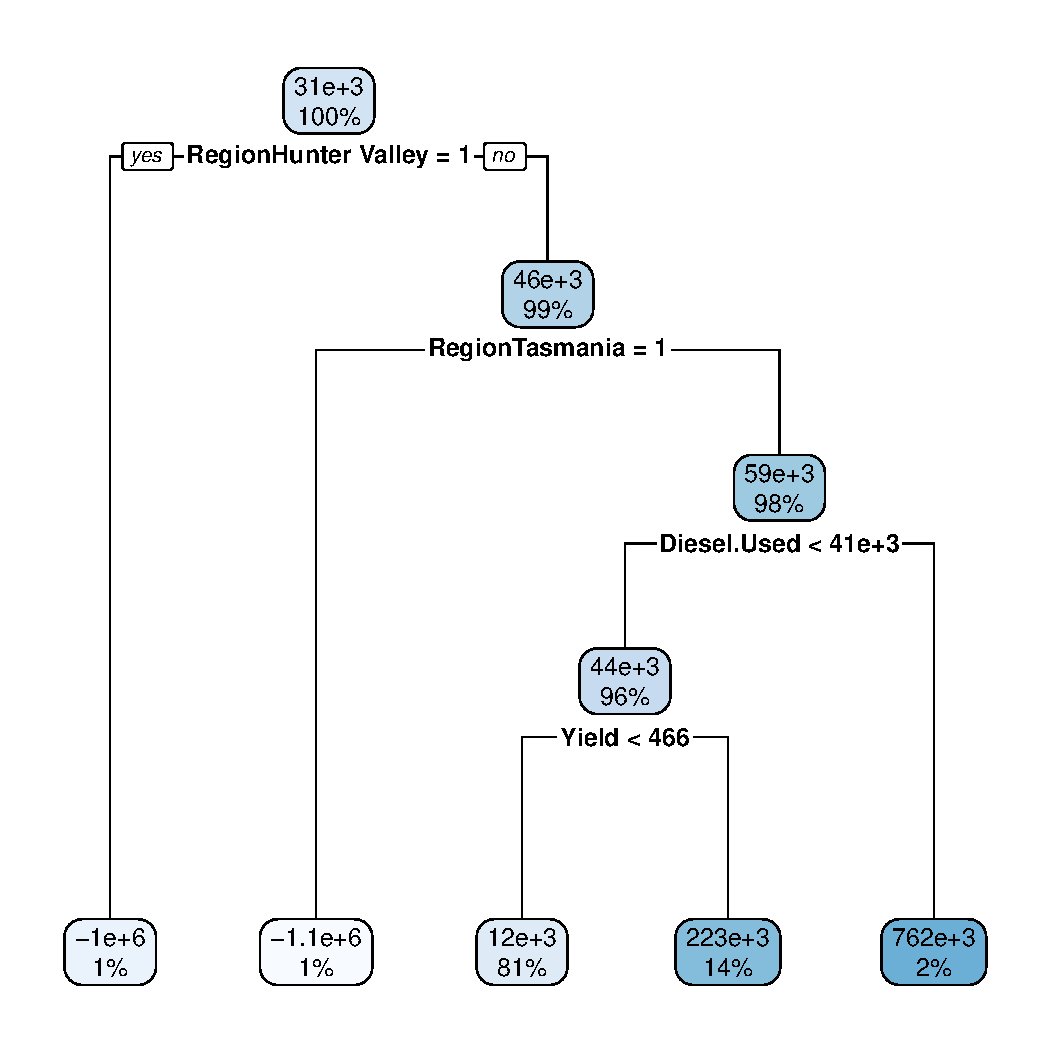
\includegraphics{profit.pdf}}
 \caption{Decision tree predicting Profit. Each node indicates the class predicted, and the proportion of elements agreeing with nodes partitioning, with the left direction indicating a yes to the nodes rule.}\label{fig:profit_tree}
\end{figure}

\begin{figure}
 \resizebox{\textwidth}{!}{
 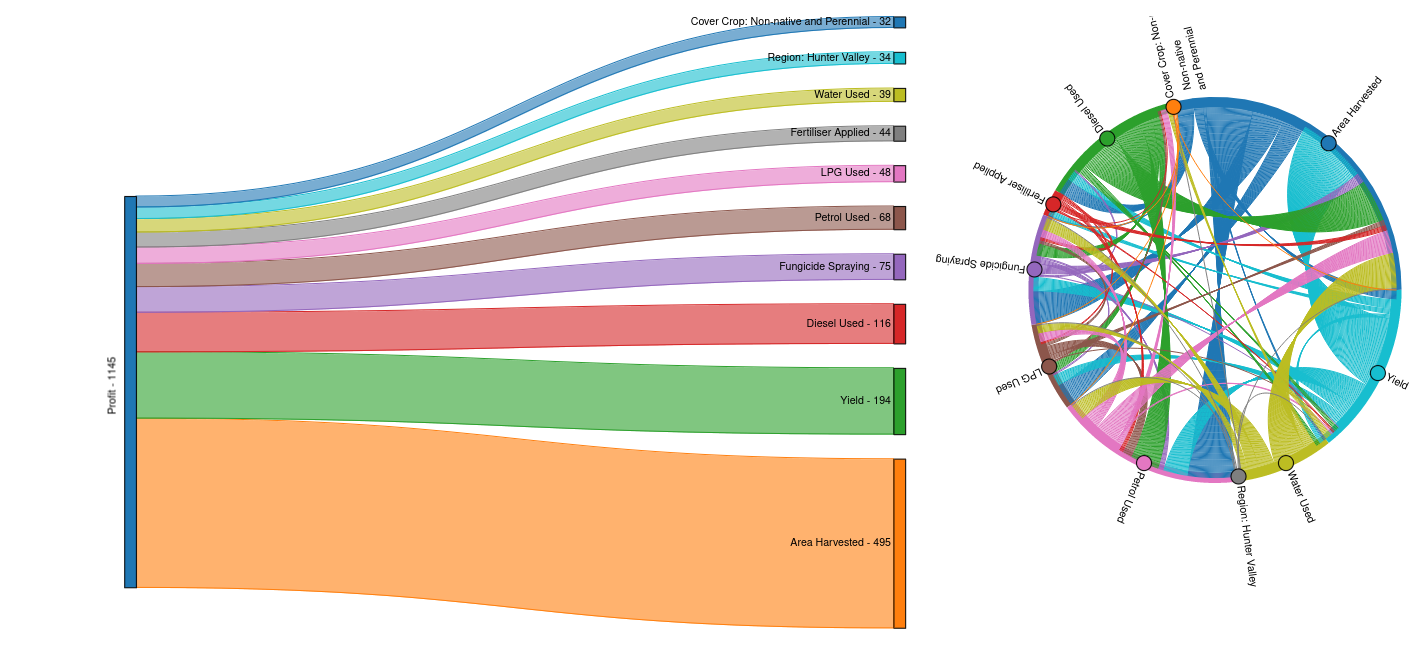
\includegraphics{profit.png}}
 % FIXME: What are the #'s? What do the sizes mean? What are the colours? What is interrelated importance?
 % FIXME: Mark one Panel A and the other B
 \caption{The left-hand side depicts the 10 most important variables in predicting Profit using XGBoosted trees as a measure of node occurrence, using a Sankey diagram. The right-hand side depicts the interrelated importance of the ten predictor variables using a chord diagram.}\label{fig:profit_sankey}
\end{figure}

% \begin{table}[]
%  \caption{Validation and training accuracies of each multiclass variable.}
%  \begin{tabular}{@{}ccc@{}}
%  \toprule
%  \textbf{Variable} & \textbf{Validation} & \textbf{Training} \\ \midrule
%  \textbf{cover crops} & 0.364086 & 0.396418 \\
%  \textbf{water type} & 0.742097 & 0.928905 \\
%  \textbf{profitable} & 0.705882 & 0.719737 \\
%  \textbf{irrigation type} & 0.841845 & 0.847554 \\
%  \textbf{giregion} & 0.505824 & 0.568242 \\
%  \textbf{irrigation energy} & 0.746293 & 0.836405 \\
%  \textbf{data year id} & 0.422003 & 0.518059 \\ \bottomrule
%  \end{tabular}
%  \end{table}

%%%%%%%%%%%%%%%%%%%%%
% Points to address
% 
\section{Discussion}

% FIXME: Mardi again asked about whether yield was per hectare. This is areally interesting consideration - we do not look at predicting yield specifically in this though. perhaps we should be very wary about these analysis with this respect.

% FIXME: Moved here from results. Find a place for this lost puppy!
%
% It is reasonable that regions, being subjected to different rainfalls and temperatures, would require different amounts of water, and would have access to different water sources. The relation of area harvested and fuel (particularly petrol) is prominent with other predictors. Due to the wide variety of uses of petrol and diesel, it is likely that they are representative of 
% other activities within the vineyard, such as pruning and harvesting. FIXME: This is new infor tht doesnt have any context (e.g no discussion yet about what fuel may be used for)
% With predictors such as yield and area being highly interconnected as they likely operate as proxy variables to other factors, possibly other present variables.

Several physical parameters such as climate, geography and soil are predetermined by a vineyard's location; making it a widely considered key determinant of grape yield and quality \citep{abbalDecisionSupportSystem2016,agostaRegionalClimateVariability2012,fragaMultivariateClusteringViticultural2017}. 
The association between yield and region is demonstrated by its position as fourth most occurring variable within the nodes of the XGBoosted ensemble which determined region (see Figure \ref{fig:region_sankey}). % FIXME: Clunky phrasing

The association with area and region is likely a connection to the change in land costs, with inland Australian areas (particularly of lower rainfall) being substantially cheaper to buy than coastal regions, allowing larger areas to be purchased \citep{willchancellorMeasuringAustralianBroadacre2019} % FIXME: Maybe but not sure this assumption holds. It may be an artefact of the members being corporate in larger holdings. The larger percentage of blocks in the riverland are small.
\par
Regions with lower land costs are also warmer \citep{willchancellorMeasuringAustralianBroadacre2019}, which is known to be beneficial in hastening the ripening process of winegrapes \citep{webbObservedTrendsWinegrape2011}. Warmer regions are also associated with lower quality grapes, caused largely due to this hastened ripening \citep{botting1996canopy}. In general if irrigated warmer regions have been associated with lower yields due to their generally lower rainfall, which can be mitigated through applying more water \citep{campsGrapeHarvestYield2012}. % FIXME: Rework this sentance
It is likely that the combination of larger vineyards with higher water use is a determining factor in classifying regions which favour larger production of lower quality grapes; reflected through the variables' importance of water use in the XGBoost ensemble. % FIXME: Need to link lower quality to profitability.
% FIXME: Warm inland regions are close to a major source of irrigation water which means that they have always taken advantage of this to grow higher crops. Which are also extremely important to our sector.)
% FIXME: May need to explain that growers are paid @ a $ value / tonne and that the $ value varies in region.
The practice of utilising larger quantities of water for inland Australian wine crops is partly reflected in the prior use of flood style irrigation to saturate soil \citep{bgcoombeGrapeBerryDevelopment2004}. % FIXME: More likely is that they have access to large water licences (Prev used for flood irrigation) That ythey now use on vineyards.
% FIXME: Examples of regions??
This classification can be contrasted with other warmer regions of higher rainfall that use the warmer climate to concentrate their grapes, increasing the flavour profile (and thus quality) \citep{goodwinijeriepRegulatedDeficitIrrigation1992,mgmccarthyEffectCropLoad1986}. This is possibly the connection between the presence of the Hunter Valley within the XGBoost ensemble that determined profit (see Figure \ref{fig:profit_sankey}). With this connection reflecting the restriction of possible strategies employable by winegrowers between different regions. % FIXME:  No this is because the hunter valley/tasmania get paid more / tonne.
\par
In part some winegrowing strategies are restricted simply through access to water resources, being reflected through the region classification tree (see Figure \ref{fig:region_tree}). Regions are likely to have varying access to different water sources, such as those along the River Murray being able to utilise river water for crops, unlike most coastal regions which may be drawing from surgace or underground water. Similarly, the connection between region and fuel use is likely an indicator of the level of infrastructure within the region. Where, the need to pressurise irrigation systems from river water or to generate power would require larger amounts of diesel and petrol. % FIXME: Yes but this requires some explanation
\par
Operational costs showed similar importance across fuel, water and tractor use. The dominating factor of area likely played a large part in determining how costly a tractor pass would be, or in defining the ratio of water applied to the amount of vines. The node frequency was high for area but much lower in general across the other variables, which could indicate the need to be more circumstantial in determining operational costs. Although it was attempted to capture the complexity between how variables interacted when determining operational costs (see Figure \ref{fig:operating_costs_sankey}), it is likely yet more complicated. An example of how interrelated operational costs can be, is 
the optimisation of tractor passes % FIXME: What does this mean? Multiple activities with a single pass?
being shown to reduce energy use in vineyards, decreasing running costs, as well as reducing soil compaction \citep{capelloEffectsTractorPasses2019}. 
\par
Decisions made on the ground have far-reaching effects and are difficult to completely capture. A higher number of tractor passes used as a preventative measure for occurrences such as disease, may incur higher operational costs but could be critical in preventing long term losses. With factors such as erosion and soil health being difficult to capture but also influenced by tractor use \citep{capelloEffectsTractorPasses2019,capelloPermanentCoverSoil2020}. Although, performing well in $R^2$, the ability to predict operational costs is limited by the variables incorporated. Reductions in fuel, water and tractor use are obvious methods to reduce operational costs but not necessarily achievable decisions. Without fully capturing more granular activities such as the specifics of what fuel was used for, it is hard to determine what decisions specifically influence the operational costs.
\par
Although less important in the XGBoost ensembles for profit, the variables: cover crops, and number of fungicide spraying and slashing passes are likely linked to broad environmental properties of regions (see Figure \ref{fig:region_sankey} and \ref{fig:profit_sankey}). Rainfall being related to vine fungal growth, disease and weed pressure. With cover crops being an effective and sustainable method to alleviate these issues \citep{delpuechAdaptingCoverCrop2018}. % FIXME: Re-structure this sentance.
It is difficult to extrapolate findings to these methods and the reason for their use due to the broad and varying definition of the regions. Utilising the Geographical Indicator regions defined by Wine Australia \citep{wineaustraliaWineAustraliaOpenData2021} is a limitation, as it is too broad to fully capture a vineyards location and its influence on more granular variables. The reasoning for using approaches such as cover crops can be widely varying. Where, a cover crop may be employed to help increase soil water retention, reduce erosion, increase biodiversity and reduce weeds \citep{capelloEffectsTractorPasses2019,capelloPermanentCoverSoil2020,delpuechAdaptingCoverCrop2018}. However, cover crops can introduce competition with grapevines and may reduce yield depending upon the plants used and the density of the cover crop \citep{goslingLongtermChangesSoil2005,monteiroInfluenceCoverCrop2007}. A more granular definition of region may help to better discern the differences in practices, and the reason for employing them. More sophisticated models, specifically those that utilise expert opinion, may also help to capture and address the decision making process. An example is the optimisation of fungicide sprays using Bayesian models that forecast disease risk \citep{luDiseaseRiskForecasting2020}. 

% In particular There is the potential that the types of herbicides used also have a long term effect on crops, reducing the presence of microorganisms and soil health, making the area more prone to disease in the long run, becoming dependent on these sprays (Coll et al., 2011; Gosling and Shepherd, 2005).

% The classification tree shows a likely change in avaialble infrastructure across the years, with mroe current years being associated with pressurised water and more slashing and herbicide passes.

% The availability of solar panels for electrical irrigation and electrical irrigation in general

% Electricity is predominantly used for pumping and irrigation in vineyards \citep{longbottomRoleVineyardPractices2015}

% Fungicides are likely associated with higher preventive sprays when disease breaks out.

% Slashing passes are likely weed outbreaks or yearly cycles?

% %% Climate change

% %% Pests Insects and weeds
% %% Disease

% %% Electricity use and reasons for (connect to year)
% %% Fuel use and what it is used for

% Operational costs saw the only occurrence of renewable resources being included in the ten most important variables for its XGBoost ensemble. 

% %% Address yield and how predictable it is
% %% different sales markets and performance?
% %% Reasons for profit?

% The winegrowing industry holds significant importance for Australia and its economy. There exists many challenges that the industry has to contend against, 
% with disease from sources such as Mildew and Botrytis being a considerable one (Cole, 2010; Magarey et al., 1994).

The disparity in accuracy between profit and operational costs is reflective of the complexity in trying to address challenges such as climate change, disease and changing market demands \citep{wineaustraliaNationalVintageReport2020,wineaustraliaNationalVintageReport2021,wineaustraliaNationalVintageReport2022}. The difference between turning a profit or loss is dependent on decisions made and chance. The difference between vineyards that make profit and those that do not could be a multitude of factors including differences in farming practices not captured within this study. Some decisions leading to latent effects such as large scale soil deposition in extreme rain events can be caused by soil compaction due to overworking a vineyard \citep{capelloPermanentCoverSoil2020}. 

\iffalse
%%%%%%%%%%%%%%%%%%%%%%%%%%%%%%%%%%%%%%%%%%%%%%%%%%%%%%%%%%%%%%%%%
%  Prior studies have shown that decisions can also have long-lasting positive effects at the cost of short term negatives. In particular the use of cover crops and remedial soil techniques offer such as trade. 

% with well established a cover crops requiring greater water resources to maintain but offering more protection in return (Capello et al., 2019; Delpuech and Metay, 2018; Gosling and Shepherd, 2005; Monteiro and Lopes, 2007). 

% Prior studies have placed an emphasis on optimisations of fungicide sprays through the development of Bayesian models to forecast disease risk (Lu et al., 2020). This analysis investigates at the synergy between spray strategies as a proxy of fuel use to different types of water sources and sustainable strategies with an emphasis on the use of cover crops; allowing for the modelling of interactions between the use of multiple strategies. With the need to balance yield, quality, and combat adversities such as disease; the creation of tools to inform decisions and assist growers with warnings of disease risks is becoming crucial in ensuring sustainable and profitable wine production (Abbal et al., 2016).

% Soil is an important and ongoing consideration for vineyards and interacts with every other practice in various ways at different time scales. For example, cover crops have been shown to be detrimental for soil health in the short term, giving an initial reduction in soil potassium and phosphorus concentrations and no change in nitrogen levels (Gosling and Shepherd, 2005). Conversely, in longer time frames the presence of a cover crop can induce an increase in microorganisms, which can excrete phosphates and potassium, regenerating the soils chemical balance and helping to introduce further organic nitrogen (Coll et al., 2011). The studies that showed this were based in two different countries of similar climate but could have been subject to other underlying conditions not measured. 

% When implementing practices such as cover crops the extent of the practice, the compounding effects and potential alternatives need to also be considered. Alternative options are always available such the use of mulch and wood chips to increase soil health and water retention in place of more involved processes such as crop rotation (Rössert et al., 2022). Crop rotation offers greater benefits than other soil management plans (Brock et al., 2011), however this is often not a viable option for many vineyards although is common practice in some places (Russo et al., 2021). The need to look at the holistic outcomes and interactions of these practices is paramount, however with the existence of many different practices, the outcomes due to interactions are not always known; one such consideration is the use of fungicide and its potential to build up copper, causing a reduction of microorganisms in the soil. Linking copper build up to any particular cause is a difficult endeavour due to the need for multiple reliable soil samples which are equally effected by the same conditions, within soil (Wightwick et al., 2010). 

% Reasons for operational costs (connect to disease and pests)

% There are several environmental concerns that affect viticulture, including loss of soil quality, lack of rain, hail, disease, fire, and frost; with climate change exacerbating these issues. In 2020, 40,000 tonnes of grapes were lost across 18 different wine regions due to bush fires and smoke taint; the predicted incidence of wildfires is expected to increase (Canadell et al., 2021). In comparison to countrywide pressures such as drought, this damage made up only 3\% of the total amount of grapes for that year; although acknowledged as a considerable loss on an individual basis, it was deemed to be only a minor national concern by Wine Australia when compared to other environmental pressures such as drought (Wine Australia, 2020). 

% In rainfed areas due to the lack of irrigation possibilities The result would be a shortening of the ripening period, with harvest occurring during the period with high temperatures, which could have a negative impact on wine quality (Salazar Parra et al. 2010; Duchne and Schneider 2005; Jones and Davis 2000) and yield (Mira de Ordua 2010; Iglesias et al. 2010).

% Climate change in the future might move the north and south latitude boundaries of areas suitable for good quality wines (Schultz and Jones 2010), and could even lead to improvements in fruit production and quality in some areas (Olesen and Bindi 2002). However, other areas may be negatively affected by high temperatures and water stress due to a reduction in the amount of water available. 


% %% Grape quality

% The difference between grape quality is most notable between warm inland regions and coastal regions such as the Riverland and Coonawarra, respectively. Grape quality is only described by a singular variable within this study, however in reality it is driven by market demand and subject to complex forces such as international market pressure, fire, pests and disease (Wine Australia, 2022, 2021, 2020, 2019; Winemakers’ Federation of Australia, 2018, 2017, 2016, 2015, 2014, 2013, 2012).

% The decision trees were able to offer some insights into the factors that influence grape quality and regional contrasts that contribute to different qualities. The most prominent being what readily available resources of each region were, particular the types of water available. Heavy water consumption is often linked to the mass production of grapes, where lower quality grapes are targeted in a quantity over quality strategy. These types of business decisions are unfortunately obfuscated by lack of in-depth data regarding vineyard business plans. Notably the literature shows that there are many complex decisions to be made on the ground depending on many compounding factors that influence both quality and yield ((Abad et al., 2021; Cortez et al., 2009; Hall et al., 2011; I. Goodwin, et al., 2009; Kasimati et al., 2022; Oliver et al., 2013; Srivastava and Sadistap, 2018)). There are also further differences when comparing winegrowers to other agricultural industries as they are vertically integrated within the wine industry, tying them to secondary and tertiary industries, such as wine production, packaging, transport and sales. This results in unique issues, where on-the-ground choices are influenced by other wine industry’s decisions, such as the use of sustainable practices in vineyards to sell in overseas markets; notably these interactions are further complicated by some winegrowers being totally integrated into wine companies, while others are not (Knight et al., 2019). It is incredibly difficult to attribute external business decisions to produced grape quality but it is important to acknowledge that some growers are contracted to produce grapes of a particular grade; it is difficult to know whether another consumer may have graded the grape quality differently paying more or less for the same grapes given the opportunity to purchase them. It is difficult to untangle the contributing factors to the success of winegrowers and the quality of grapes produced without further specifics of choices made through out a season (Leilei He et al., 2022).

% %% connection to watrer resource availability
% What are the water resources in the hunter valley and tasmania?

% economic pressures

% Historically strong demands for Australian wine have helped to create a thriving industry, however recently sharp reductions in exports to mainland China due to significant deposit tariffs have caused a decline of 19% in Australian export value during the 2021-2022 financial year (see Figure 1) (Wine Australia, 2022). The pressure brought on by the drop in export value has been exacerbated by loss of tourism and labour due to the COVID-19 pandemic, global freight crisis, war in Europe and rising inflation (Wine Australia, 2021a, 2020). These pressures within the wine industry have trickled down to vineyards, where winemakers retain unwanted wine, creating an oversupply of grapes. Currently the proposed strategy to soften pressures proposed by Wine Australia includes initiatives focused on market diversification, and sustainability to build resilience in the coming years. 

% Figure 1: The exports of Australian wine over time in Australian Dollars Free On Board, comparing exports between China and the rest of the world. This graphic is taken from the Wine Australia Annual Report of 2020-21(Wine Australia, 2022).

%%%%%%%%%%%%%%%

% %Two regions, the Riverland and Coonawarra, were the most accurate classes being 92.74% and 96.97% respectively. 

% These regions differ greatly in practice and geophysical properties, with the Riverland being a dry warm inland region and Coonawarra being a cooler, wet coastal region. However, they are both similar in operational scales, with vineyards being relatively large compared with other regions. The differences in resources and practices between these regions are also significant, such as the Riverland utilising the river Murray as a water source. 

% The difference between grape quality is most notable between warm inland regions and coastal regions such as the Riverland and Coonawarra, respectively. Grape quality is only described by a singular variable within this study, however in reality it is driven by market demand and subject to complex forces such as international market pressure, fire, pests and disease \citep{wineaustraliaNationalVintageReport2019,wineaustraliaNationalVintageReport2020,wineaustraliaNationalVintageReport2021,wineaustraliaNationalVintageReport2022,winemakersfederationofaustraliaNationalVintageReport2015,winemakersfederationofaustraliaNationalVintageReport2016,winemakersfederationofaustraliaNationalVintageReport2017,winemakersfederationofaustraliaNationalVintageReport2018} % The original citation included years prior to this dataset just be casreful with this. It is a bit unclear what you are really trying to cite and its relevance. I think it important to chop this up.

% The decision trees were able to offer some insights into the factors that influence grape quality and regional contrasts that contribute to different qualities. The most prominent being what readily available resources of each region were, particular the types of water available. 
% A citation or reference to a study looking at the disparity in wine regions and their resources - or use the data more to describe these regional differences. Is water availability apparent? Do some regions have access to more sohpisticated water sources such as pressurised water etc.

%  Heavy water consumption is often linked to the mass production of grapes, 
 
 % Really? proce it? Where in the results is this really found?? This sounds like a link to your previous paper but you cannot really show this and you do not really produce evidence to support this claim.

%  where lower quality grapes are targeted in a quantity over quality strategy. These types of business decisions are unfortunately obfuscated by lack of in-depth data regarding vineyard business plans. 

 % This point is incredibly important but it, itself, is obfuscated by you odd claims that are not supported by facts. Better to talk about how this could improve and the weaknesses than to start spouting unsupported claims.

%  Notably the literature shows that there are many complex decisions to be made on the ground depending on many compounding factors that influence both quality and yield \citep{abadCoverCropsViticulture2021,cortezUsingDataMining2009,hallWithinseasonTemporalVariation2011,i.goodwinManagingSoilWater2009,kasimatiPredictingGrapeSugar2022,oliverReviewSoilPhysical2013,srivastavaNondestructiveSensingMethods2018}
 % Woah woah woah
%
 % what are these decisions??? Slow down speed gonzales!! This is really interseteing and important. Discuss it, its the discussion! God damn I want to know and I wrote this!.
 %
%
% This is not all one paragraph surely! There are so many ideas here that should be discussed!
%
% This leads heavily into the next paper and shows that natural progression. Especially in the sense of: if regions have so much influences, what determines ones use of water, fertiliser, etc. And, what determines the success financially, in quality or quantity? How are thes evariables interacting! The next paper is less about predicting and much more about what interacts with what? Where as this paper is about how things change over landscapes and what localised events helpe to determine decisions and their outcomes.
%
%  . There are also further differences when comparing winegrowers to other agricultural industries as they are vertically integrated within the wine industry, tying them to secondary and tertiary industries, such as wine production, packaging, transport and sales. This results in unique issues, where on-the-ground choices are influenced by other wine industry's decisions, such as the use of sustainable practices in vineyards to sell in overseas markets; notably these interactions are further complicated by some winegrowers being totally integrated into wine companies, while others are not (Knight et al., 2019). 

% This is an interesting point. However it would be better to include other industries, such as the ones you touch on in your previous chapter. If industries such as Sake are similar - how do their decisions effect the outcomes of rice quality and Sake? A point of comparison and difference would be great here! 

%  It is incredibly difficult to attribute external business decisions to produced grape quality but it is important to acknowledge that some growers are contracted to produce grapes of a particular grade; it is difficult to know whether another consumer may have graded the grape quality differently paying more or less for the same grapes given the opportunity to purchase them.

% What are these business decisions? Can you give some examples?

%  It is difficult to untangle the contributing factors to the success of winegrowers and the quality of grapes produced without further specifics of choices made through out a season \citep{leileiheFruitYieldPrediction2022}.

% It is difficult yes, but please at least try! Highlight some of these affects, some of these different contributing factors! What did we really learn by doing this? What can someone take away from this and say thank you for? (like Josh said)


% \subsection{Model 1 GI Regions}

% The first Model was used to classify GI regions
 % Interestingly the firs I am hearing of this - each model needs to be more well summarised. A table would be good.

% and resulted in an accuracy of 36.48\% across 52 classes. The most prominent features used to classify regions were the types of water resources available (see Figure 1). Two regions, the Riverland and Coonawarra, were the most accurate classes being 92.74\% and 96.97\% respectively.

% it might be worth only talking about the regions that were well classifified - and then talk about their determining traits.

% These regions differ greatly in practice and geophysical properties, with the Riverland being a dry warm inland region and Coonawarra being a cooler, wet coastal region. However, they are both similar in operational scales, with vineyards being relatively large compared with other regions.

%Summary statistics regarding these two regions would be a better point of comparison, for example:
%
% How much in size do these operational scales differ?
% How much yield do they differ by?
% What are the differences in rainfall etc
% What makes them unique, different and similar?
%

% The differences in resources and practices between these regions are also significant, such as the Riverland utilising the river Murray as a water source.
% What are the specific differences? This is a really critical part of this paper

% Many of the regions had significantly lower reporting rates, resulting much poorer classification performance.
 % This is almost its own paragraph. Why was this case? is it important? what are the similarities and differences of regions that were poorly classified?

%  The regions with the most samples performed the best (see Table 1). Notably bordering regions were routinely grouped together and misclassified as the same region, for example the two closest regions to Coonawarra, Padthaway and Wrattonbulley, were misclassified as Coonawarra even though they had 147 and 137 samples respectively. The same case was found for the Murray Darling, with 143 samples, it was misclassified as the Riverland.
 % This speaks highly to why regions were poorly classified.

% These misclassifications are likely due to the incredibly similar regional properties and close proximity these regions have with one another. Other misclassifications were most likely due to lower reporting rates with many regions being under represented.

% \begin{table}[]
%   \caption{Classification accuracy of the most prominent GI Regions.}
%   \label{tab:accuracy}
%   \resizebox{\textwidth}{!}{
%     \begin{tabular}{@{}llll@{}}
%       \toprule
%       \textbf{} & \textbf{Accuracy} & \textbf{Predicted} & \textbf{Actual} \\ \midrule
%       \textbf{Adelaide Hills} & 30.45\% & 95 & 312 \\
%       \textbf{Barossa Valley} & 51.00\% & 205 & 402 \\
%       \textbf{Coonawarra} & 96.97\% & 192 & 198 \\
%       \textbf{Langhorne Creek} & 22.84\% & 53 & 232 \\
%       \textbf{Margaret River} & 78.82\% & 201 & 255 \\
%       \textbf{McLaren Vale} & 52.89\% & 128 & 242 \\
%       \textbf{Riverland} & 92.74\% & 345 &
%     \end{tabular}
%   }
% \end{table}

% \subsection{Climate}
% Classifying the SWA climatic categorisation of the given regions had better performance than the GI Regions, with ~41.66\% being classified correctly. These categories were divided into 12 climatic classifications with 3 and 4 separate subsets for rainfall and temperature respectively. The decision tree behaved similarly and over classified climates with higher response rates. The results posed an interesting similarity with grape quality classifier, being influenced predominantly by water and area. The use of fungicide to separate regions that were 'Very dry' and 'Damp' can be considered as indicative of the different practices required due to climatic pressure; fungicides being more prominent in cooler regions with greater rainfall due to the higher risk of disease pressure \citep{reynoldsManagingWineQuality2010}. % interesting although not really appropriate for the results section.
%  This could also potentially explain the use of contractor tractor use to discern differences in grape quality, where the lack of contractor use to prevent disease could have led to lowered quality of grapes.

% You really need to show every decision tree.

% \subsubsection{Rainfall}
% The rainfall decision tree showed a greater use of fungicides sprays to discern between damp and very Dry as shown in Figure 4; with the accuracy improving to 62\% but was unable to effectively discern between dry and very dry regions (see Table 3).

% was again used to differentiate between warm and cool regions, likely being due to disease pressure. The temperature classification tree

% \subsection{Model 3 Grape Quality}
% The classification of grape quality through its grade % It might even be worth considering this as pseudo grade - or better define it in some of the australian wine journals rose suggested.
% had an accuracy of 55.72\% across 5 separate grades. There was a notable issue with the classification of B grade grapes when compared to A and C (see Table 2). % This is actually really interesting.
%  The classification tree itself shows similarities to that of classifying regions in Model 1, with the type of water resource used being a prominent determiner. Although not surprising the number of contractor tractor passes is new deciding factor due disease and pests reducing the potential quality of a crop. The prevalence of contractor use is greater in regions such as the Barossa Valley and the McLaren Vale, this could be due to the difference in operational scales, with larger sites being more likely to have ownership of their own equipment for weeding and spraying due to the cost benefit.

\fi

\section{Conclusion}

This study has provided valuable insights into the multifaceted dynamics governing operational costs, different yearly effects and vineyard regions highlighting the complex interrelatedness of variables within a vineyard. The paper underscores how factors such as water and fuel intersect to impact operational costs and How different seasonal events affect these operations and the significance of context-specific decision-making. While this investigation utilised a broad regional classification, the potential benefits of adopting a more nuanced approach and incorporating expert knowledge have been highlighted. By delving deeper into the complex interplay of variables, further advancements can be made in optimising vineyard management strategies for lowering operational costs and enhancing sustainability.

% The intricate relationships between water resources, and management practices have been examined through advanced techniques like XGBoost ensembles, shedding light on their roles in shaping production outcomes.


% The type and availability of water resources were a major contributing factor when classifying grape quality and region. This was seen in the two most accurately classified regions, Coonawarra and the Riverland, with the Riverland predominantly utilising river water. Furthermore, the study highlighted the influence of water use, fungicide application, and contractor use in differentiating grape quality, climate and region respectively. These models provide insight into the complex dynamics between regional characteristics, sustainable practices, and grape quality in the Australian winegrowing industry. It is important to acknowledge that grape quality is subject to external influences such as market demands and prior established business arrangements. Further in-depth data and understanding are necessary to fully grasp the nuances of decision-making and the interplay of factors impacting grape quality.

% Interesting - the conclusion is actually reasonable, especially considering the disconnection of ideas and models in this paper.

%%%%%%%%%%%%%%%%%%%%%%%%%%%%%%%%%%%%%%%%%%
%%       End Matter       %%
%%%%%%%%%%%%%%%%%%%%%%%%%%%%%%%%%%%%%%%%%%

\bibliography{references} % This points to the references.bib file - the file extention is automatically added.
\bibliographystyle{elsarticle-harv}

%% The Appendices part is started with the command \appendix;
%% appendix sections are then done as normal sections
 \appendix


 \subsection{Year}

 The classification tree and XGBoosted ensemble performed similarly for classifying year with 35.20\% (6.28\% standard deviation) and 51.81\% (42.20\% validation accuracy) respectively. Electricity and the type of irrigation were highly influential within the classification tree. Similarly, electricity was the most frequently occurring node in the XGBoost ensemble. Other variables such as slashing passes, and fungicide and herbicide spraying were more prevalent than in the classification tree. Weed and disease outbreaks are likely an influential factor when classifying different years, making the decisions to spray and slash unique factors that differ year to year. Climatic differences between years are likely tied to the influence of yield and water use.
 \par
 Over half of the interrelated importance of the predictor variables is dominated by area harvested, yield and slashing passes. Although all the predictor variables are highly connected, their relative importance is not as prominent as the three major variables. It is of particular note of the relative importance of slashing passes to area, fuel and yield; as these are not directly related activities. The connection between the number of slashing and spraying passes is that those who do a set number of spraying or slashing passes tended to do that many passes for all slashing and spraying activities.
 
 \begin{figure}
  \resizebox{\textwidth}{!}{
  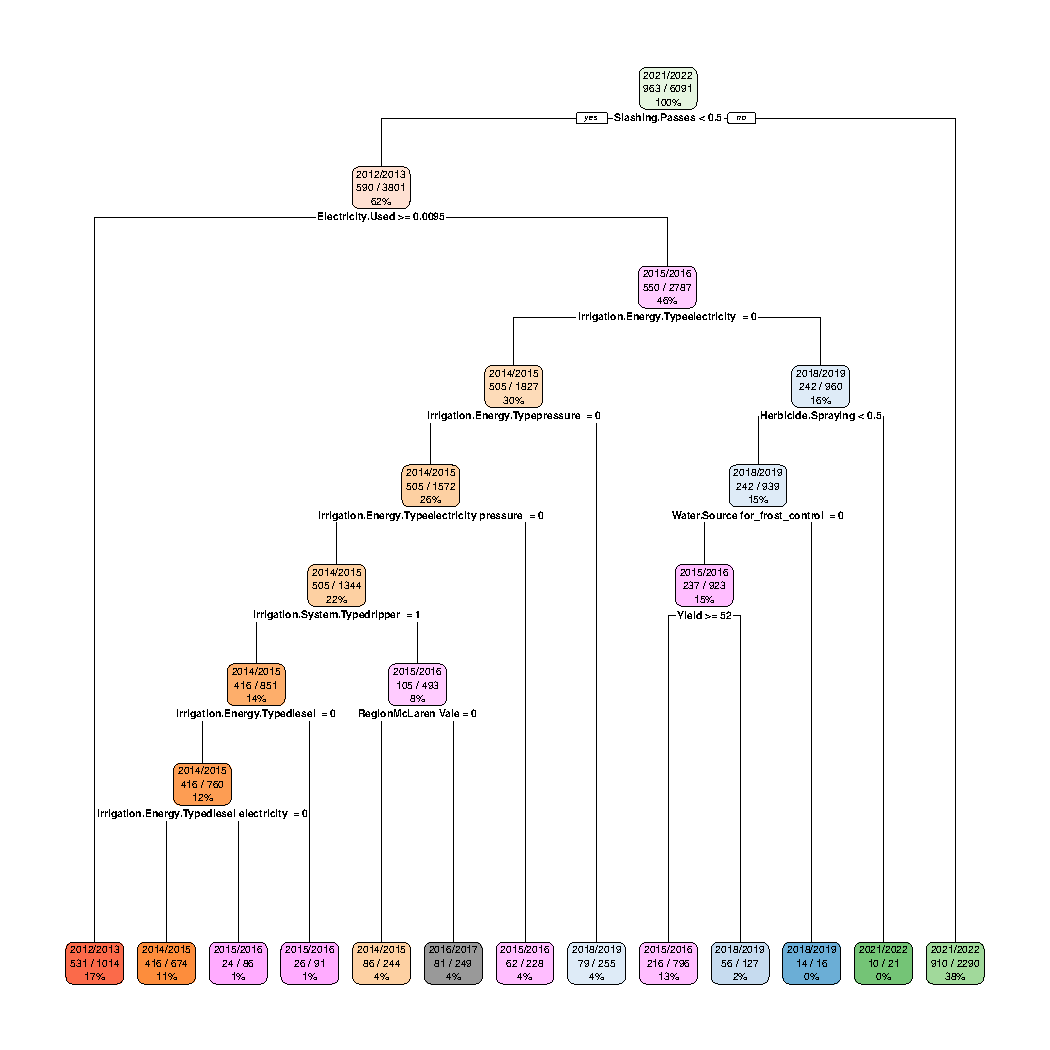
\includegraphics{year.pdf}}
  \caption{Decision tree predicting Year. Each node indicates the class predicted, and the proportion of elements agreeing with nodes partitioning, with the left direction indicating a yes to the nodes rule.}\label{fig:year_tree}
 \end{figure}
 
 \begin{figure}
  \resizebox{\textwidth}{!}{
  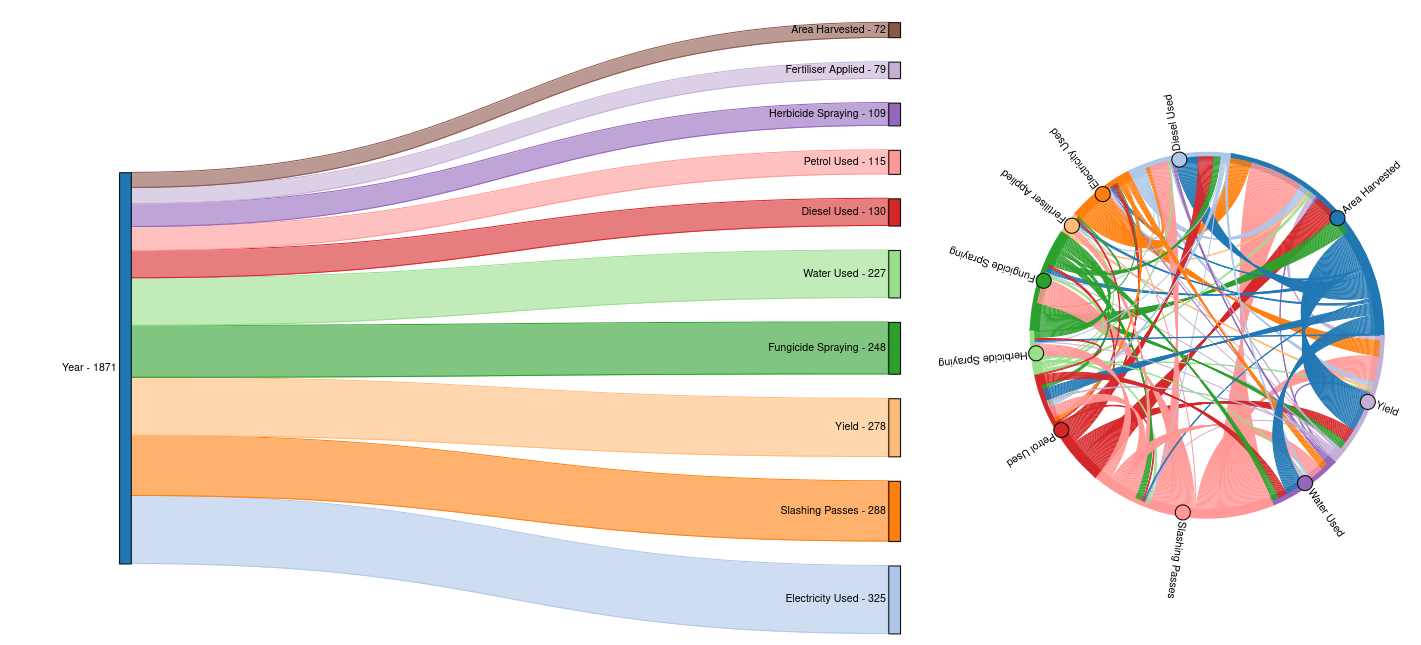
\includegraphics{year.png}}
  \caption{The left-hand side depicts the 10 most important variables in predicting Year using XGBoosted trees as a measure of node occurrence, using a Sankey diagram. The right-hand side depicts the interrelated importance of the ten predictor variables using a chord diagram.}\label{fig:year_sankey}
 \end{figure}
 

\end{linenumbers}
 \end{document}
 
\endinput
